\documentclass[11pt,a4paper]{article}

\usepackage[utf8]{inputenc}
\usepackage[T1]{fontenc}
\usepackage{amsmath,amssymb,amsthm}
\usepackage{mathtools}
\usepackage{bm}
\usepackage{booktabs}
\usepackage{graphicx}
\usepackage{hyperref}
\usepackage[margin=2.5cm]{geometry}
\usepackage{caption}
\usepackage{enumitem}
\usepackage{xcolor}
\usepackage{mdframed}
\usepackage{array}
\usepackage{float}
\graphicspath{{figures/}}

\newtheorem{theorem}{Theorem}[section]
\newtheorem{lemma}[theorem]{Lemma}
\newtheorem{proposition}[theorem]{Proposition}
\newtheorem{corollary}[theorem]{Corollary}
\theoremstyle{definition}
\newtheorem{definition}[theorem]{Definition}
\newtheorem{remark}[theorem]{Remark}

\newcommand{\R}{\mathbb{R}}
\newcommand{\E}{\mathbb{E}}
\newcommand{\Var}{\operatorname{Var}}
\newcommand{\rms}{\operatorname{rms}}
\newcommand{\relu}{\operatorname{ReLU}}
\DeclareMathOperator{\tr}{tr}
\DeclareMathOperator*{\argmin}{arg\,min}

\newenvironment{flagbox}{%
  \begin{mdframed}[linecolor=blue!75!black,backgroundcolor=blue!5!white,linewidth=1.5pt]%
  \textbf{\textcolor{blue!75!black}{Key Result.}}\ %
}{%
  \end{mdframed}%
}

\title{%
  Gradient-Product-Balanced Initialization\\[4pt]
  {\large A Per-Layer Variance Schedule for Row-Centered ReLU Networks}
}
\author{Itay Ofer}
\date{April 2026}

\begin{document}
\maketitle
\tableofcontents
\newpage

%======================================================================
\section{Goal and Motivation}
\label{sec:motivation}

We seek an initialization scheme for deep ReLU networks that simultaneously:
\begin{enumerate}[nosep]
  \item \textbf{Preserves geometry} --- class separability should survive deep projections.
  \item \textbf{Maintains gradient stability} --- gradient magnitudes should be approximately uniform across layers.
\end{enumerate}

From BP4, the gradient of the loss $\mathcal{C}$ at layer~$\ell$ is:
\begin{equation}\label{eq:bp4}
  \frac{\partial \mathcal{C}}{\partial W^{(\ell)}}
  = \frac{1}{n}\bigl(\Delta^{(\ell)}\bigr)^{\!\top}\! A^{(\ell-1)},
\end{equation}
where $A^{(\ell-1)} \in \R^{n \times d_{\ell-1}}$ is the activation matrix
(input to layer~$\ell$) and $\Delta^{(\ell)} \in \R^{n \times d_\ell}$ is the error signal matrix.
Taking Frobenius norms:
\begin{equation}\label{eq:grad-mag}
  \left\|\frac{\partial \mathcal{C}}{\partial W^{(\ell)}}\right\|_F
  \;\propto\; \rms\!\bigl(A^{(\ell-1)}\bigr) \cdot \rms\!\bigl(\Delta^{(\ell)}\bigr).
\end{equation}

This product depends on two per-layer quantities:
\begin{itemize}[nosep]
  \item \textbf{Forward gain:}
    $g_{\mathrm{fwd}}^{(\ell)} = \rms(A^{(\ell)}) / \rms(A^{(\ell-1)})$
    --- how the signal changes layer to layer.
  \item \textbf{Backward gain:}
    $g_{\mathrm{bwd}}^{(\ell)} = \rms(\Delta^{(\ell)}) / \rms(\Delta^{(\ell+1)})$
    --- how the error signal changes backward.
\end{itemize}
We define the \textbf{gradient ratio} as
$\max_\ell \|\nabla_{W^{(\ell)}}\mathcal{C}\|_F \;/\;
 \min_\ell \|\nabla_{W^{(\ell)}}\mathcal{C}\|_F$.
A ratio of~1 means perfectly uniform gradients.


%======================================================================
\section{Forward and Backward Gains for Row-Centered Weights}
\label{sec:gains}

\subsection{Setup and notation}

Consider a layer with row-centered weight matrix $W \in \R^{d \times d}$,
meaning $\sum_j W_{ij} = 0$ for every row~$i$.  The per-element variance
is $\Var(W_{ij}) = v/d$.  We define a convenient \textbf{variance factor}:
\begin{equation}\label{eq:s-def}
  s = \sqrt{\frac{v}{2}}.
\end{equation}
When $s = 1$, we recover standard He variance ($v = 2/d \cdot d = 2$, i.e., $\Var(W_{ij}) = 2/d$).

\subsection{Forward gain: why row centering loses signal}
\label{sec:fwd-derivation}

The key question: how much output energy $\E[(a^{(\ell)})^2]$ does a
layer produce, given input energy $\E[(a^{(\ell-1)})^2]$?

\textbf{Without row centering} (standard He), the answer is well known.
Each neuron computes $z_i = \sum_j W_{ij}\,a_j$, and the variance of~$z_i$ is:
\[
  \Var(z_i) = d \cdot \Var(W_{ij}) \cdot \E[a_j^2] = v \cdot \E[a^2].
\]
After ReLU (which zeroes out $\sim\!50\%$ of values), the output energy is
$\E[(a^{(\ell)})^2] = \frac{v}{2} \cdot \E[(a^{(\ell-1)})^2]$.
He sets $v = 2$, giving $\E[(a^{(\ell)})^2] = \E[(a^{(\ell-1)})^2]$: forward gain $= 1$.

\textbf{With row centering}, the neuron output changes.
Since $\sum_j W_{ij} = 0$, we can write:
\[
  z_i = \sum_j W_{ij}\,a_j = \sum_j W_{ij}\,(a_j - \bar{a}),
  \qquad \bar{a} = \tfrac{1}{d}\sum_k a_k.
\]
The constant part $\bar{a} \cdot \sum_j W_{ij}$ vanishes.  The neuron only
``sees'' the deviations $a_j - \bar{a}$, not the mean~$\bar{a}$.

Now, post-ReLU activations $a = \relu(z)$ with $z \sim \mathcal{N}(0, \sigma^2)$
have a positive mean:
\[
  \E[a] = \frac{\sigma}{\sqrt{2\pi}} > 0, \qquad
  \E[a^2] = \frac{\sigma^2}{2}, \qquad
  \Var(a) = \E[a^2] - (\E[a])^2 = \frac{\sigma^2(\pi-1)}{2\pi}.
\]
The fraction of energy in the deviations (what row-centered weights can access) is:
\begin{equation}\label{eq:centering-ratio}
  \frac{\Var(a)}{\E[a^2]} = \frac{\pi-1}{\pi} \approx 0.682.
\end{equation}
This is a universal property of ReLU --- independent of~$\sigma$ or~$d$.

Since row-centered weights see $\Var(a)$ instead of $\E[a^2]$, the output energy becomes:
\[
  \E[(a^{(\ell)})^2] = \frac{v}{2} \cdot \frac{\pi-1}{\pi} \cdot \E[(a^{(\ell-1)})^2]
                      = s^2 \cdot \frac{\pi-1}{\pi} \cdot \E[(a^{(\ell-1)})^2].
\]
Taking square roots for the forward gain:
\begin{equation}\label{eq:fwd-gain}
  \boxed{\;g_{\mathrm{fwd}} = r \cdot s,
  \qquad r = \sqrt{\frac{\pi-1}{\pi}} \approx 0.826.\;}
\end{equation}
The factor~$r$ is structural: it comes from row centering being blind to the
mean of post-ReLU activations.  No variance adjustment can remove it.

\subsection{Backward gain: why the backward pass is unaffected}
\label{sec:bwd-derivation}

The backward pass computes
$\bm{\delta}^{(\ell)} = (W^{(\ell+1)})^\top \bm{\delta}^{(\ell+1)} \odot \sigma'(\bm{z}^{(\ell)})$,
where $\sigma'(\bm{z}^{(\ell)}) = \mathbf{1}[z^{(\ell)} > 0]$ is the ReLU derivative
(binary mask).

Row centering of~$W$ means $\sum_j W_{ij} = 0$ (rows sum to zero).  The
transpose $W^\top$ therefore has $\sum_i W_{ij} = 0$ (columns sum to zero).
By the same logic as the forward pass, $W^\top$ is blind to the mean of
its input $\bm{\delta}^{(\ell+1)}$.

However, unlike post-ReLU activations, the error signal
$\bm{\delta}$ contains both positive and negative values, so its mean
is near zero: $\Var(\delta)/\E[\delta^2] \approx 1$.  There is
almost no ``DC component'' to lose.

Therefore the backward gain depends only on the weight scale:
\begin{equation}\label{eq:bwd-gain}
  \boxed{\;g_{\mathrm{bwd}} = s.\;}
\end{equation}

\subsection{The coupling}
Dividing \eqref{eq:fwd-gain} by \eqref{eq:bwd-gain}:
\begin{equation}\label{eq:coupling}
  \frac{g_{\mathrm{fwd}}}{g_{\mathrm{bwd}}} = r \approx 0.826,
  \qquad\text{always, regardless of } s.
\end{equation}
No single scalar variance can make both gains equal to~1 simultaneously.


%======================================================================
\section{The Product-Balanced Initializer}
\label{sec:product-balanced}

\subsection{Derivation}
Since we cannot achieve $g_{\mathrm{fwd}} = g_{\mathrm{bwd}} = 1$,
we seek the next best thing: $g_{\mathrm{fwd}} \cdot g_{\mathrm{bwd}} = 1$.

\begin{theorem}[Product-balanced variance]
  \label{thm:product-balanced}
  The unique~$s^{\ast}$ satisfying $g_{\mathrm{fwd}} \cdot g_{\mathrm{bwd}} = 1$ is
  \begin{equation}\label{eq:s-star}
    s^{\ast} = \left(\frac{\pi}{\pi-1}\right)^{\!1/4} \approx 1.1006,
    \qquad
    \Var(W_{ij}) = \frac{2\sqrt{\pi/(\pi-1)}}{d} \approx \frac{2.422}{d}.
  \end{equation}
\end{theorem}
\begin{proof}
  $g_{\mathrm{fwd}} \cdot g_{\mathrm{bwd}} = r s \cdot s = r s^2 = 1$
  $\;\Longrightarrow\;$ $s^2 = 1/r = \sqrt{\pi/(\pi-1)}$
  $\;\Longrightarrow\;$ $s^{\ast} = (\pi/(\pi-1))^{1/4}$.
\end{proof}

Resulting gains: $g_{\mathrm{fwd}}^{\ast} = ((\pi-1)/\pi)^{1/4} \approx 0.909$,
$\;g_{\mathrm{bwd}}^{\ast} = (\pi/(\pi-1))^{1/4} \approx 1.101$,
$\;g_{\mathrm{fwd}}^{\ast} \cdot g_{\mathrm{bwd}}^{\ast} = 1$ (exact).

\subsection{Initialization procedure}
\begin{definition}[Product-balanced row-centered initialization]
\label{def:init-uniform}
Given a layer with fan-in~$d$:
\begin{enumerate}[nosep]
  \item Set $\sigma = \sqrt{2\sqrt{\pi/(\pi-1)} \;/\; d}$.
  \item Sample $W_{ij} \sim \mathcal{N}(0, \sigma^2)$.
  \item Row-center: $W_{ij} \leftarrow W_{ij} - \frac{1}{d}\sum_k W_{ik}$.
  \item Rescale each row: $\bm{w}_i \leftarrow \bm{w}_i \cdot \sigma / \mathrm{std}(\bm{w}_i)$.
  \item Set bias to zero.
\end{enumerate}
\end{definition}


%======================================================================
\section{Per-Layer Variance Scaling: The $\eta$-Schedule}
\label{sec:layer-balanced}

Uniform variance cannot produce uniform gradients (as we show in
Section~\ref{sec:pareto}).  We derive a per-layer schedule from BP4.

\subsection{Derivation}
\label{sec:eta-derivation}

\textbf{Step 1 (Forward chain).}
$\rms(A^{(\ell-1)}) = \rms(A^{(0)}) \cdot \prod_{k=1}^{\ell-1} (r \cdot s_k)
                     = \rms(A^{(0)}) \cdot r^{\ell-1} \cdot \prod_{k=1}^{\ell-1} s_k$.

\textbf{Step 2 (Backward chain).}
The backward gain at position~$k$ is $g_{\mathrm{bwd}}^{(k)} \approx s_{k+1}$.
Telescoping: $\rms(\Delta^{(\ell)}) = \rms(\Delta^{(L)}) \cdot \prod_{k=\ell+1}^{L} s_k$.

\textbf{Step 3 (Gradient at layer~$\ell$).}
Substituting into \eqref{eq:grad-mag}:
\begin{equation}\label{eq:gradient-formula}
  \left\|\frac{\partial\mathcal{C}}{\partial W^{(\ell)}}\right\|
  \propto r^{\ell-1} \cdot \frac{\prod_{k=1}^{L} s_k}{s_\ell}.
\end{equation}
Since $\prod_{k=1}^L s_k$ is constant across~$\ell$:
\begin{equation}\label{eq:gradient-simple}
  \boxed{\;\left\|\frac{\partial\mathcal{C}}{\partial W^{(\ell)}}\right\|
  \propto \frac{r^{\ell-1}}{s_\ell}.\;}
\end{equation}

\textbf{Step 4 (Uniform gradients).}
$r^{\ell-1}/s_\ell = \text{const}$ requires $s_\ell \propto r^{\ell-1}$.

\subsection{The $\eta$-parameterization}
\label{sec:eta-param}

Setting $s_\ell = C \cdot r^{\ell-1}$ directly would fully correct the gradient,
but at the cost of extreme variance differences between layers (since $r < 1$,
early layers get much larger variance than late layers).  We introduce a
\emph{correction strength} $\eta \in [0,1]$:
\begin{equation}\label{eq:eta-schedule}
  s_\ell = s^{\ast} \cdot r^{\,\eta\,(\ell - (L+1)/2)},
\end{equation}
where $s^{\ast} = (\pi/(\pi-1))^{1/4}$ (the product-balanced factor) and the
exponent is centered at the middle layer so the geometric mean equals~$s^{\ast}$.

\begin{itemize}[nosep]
  \item $\eta = 0$: uniform variance, no correction.  Gradient ratio $= r^{-(L-1)}$.
  \item $\eta = 1$: full correction, perfect gradient uniformity, but variance ratio $= r^{-(L-1)}$.
  \item $0 < \eta < 1$: partial correction --- a trade-off.
\end{itemize}

The parameter $\eta$ is \textbf{not derived from theory} --- it is a tunable
knob that controls the trade-off.

\begin{definition}[Layer-balanced product-base initialization]
\label{def:init-layerbal}
For layer~$\ell \in \{1,\ldots,L\}$ with fan-in~$d_{\ell-1}$:
\begin{equation}\label{eq:target-std}
  \sigma_\ell = \sqrt{\frac{2}{d_{\ell-1}}} \cdot s^{\ast} \cdot r^{\,\eta\,(\ell - (L+1)/2)}.
\end{equation}
Then apply the same procedure as Definition~\ref{def:init-uniform},
using $\sigma_\ell$ (which varies per layer) instead of a fixed~$\sigma$.
\end{definition}


%======================================================================
\section{Empirical Validation (50 Hidden Layers)}
\label{sec:empirical}

\subsection{Setup}
Fashion-MNIST, 2000 samples, architecture $784 \to [784]^{50} \to 1$.
Four initializers compared:
\begin{enumerate}[nosep]
  \item \textbf{He} --- standard Kaiming (baseline).
  \item \textbf{RC fwd-balanced} --- $g_{\mathrm{fwd}} = 1$, $g_{\mathrm{bwd}} \approx 1.21$.
  \item \textbf{RC product-balanced} --- $g_{\mathrm{fwd}} \cdot g_{\mathrm{bwd}} = 1$ (uniform).
  \item \textbf{RC layer-balanced (product base, $\eta = 0.5$)} --- per-layer scaling.
\end{enumerate}

\subsection{Gain verification}
\begin{table}[H]
\centering
\caption{Per-layer gain comparison, 50 hidden layers.}
\label{tab:gains}
\begin{tabular}{l c c c c c}
\toprule
Initializer & Med $g_{\mathrm{fwd}}$ & Med $g_{\mathrm{bwd}}$ & Product & Grad ratio & Grad CV \\
\midrule
He (baseline) & 0.993 & 0.997 & 0.990 & 7.8$\times$ & 0.522 \\
RC fwd-balanced & 1.000 & 1.209 & 1.210 & 1901$\times$ & 1.903 \\
RC product-balanced & 0.909 & 1.099 & 0.999 & 1902$\times$ & 1.906 \\
\textbf{RC layer-bal ($\eta\!=\!0.5$)} & \textbf{0.956} & \textbf{1.049} & \textbf{1.003} & $\bm{36\times}$ & \textbf{1.095} \\
\bottomrule
\end{tabular}
\end{table}

The layer-balanced variant reduces the gradient ratio from $1902\times$ (uniform RC) to $36\times$ --- a $53\times$ improvement.  However, He's $7.8\times$ remains significantly better.

\subsection{Forward gain per layer}
\begin{figure}[H]
  \centering
  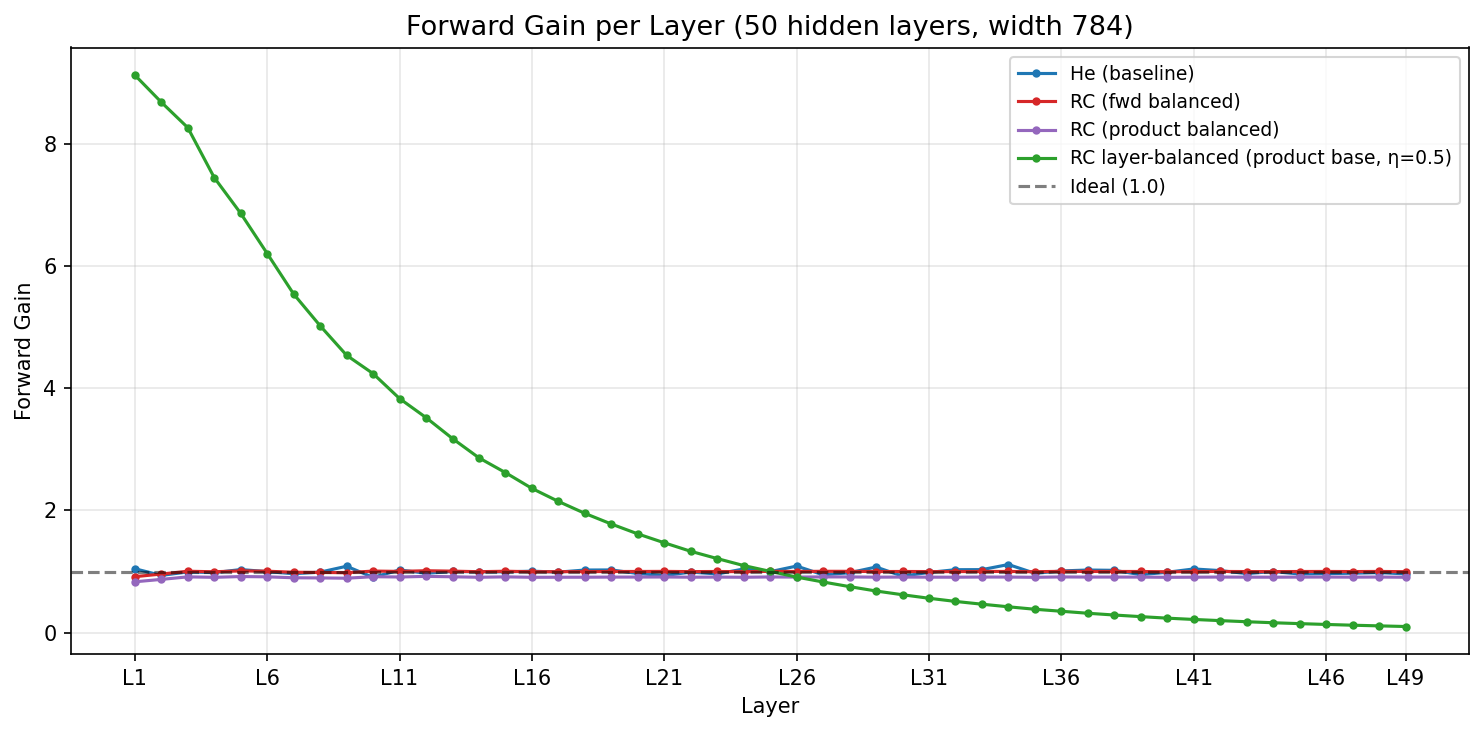
\includegraphics[width=0.92\textwidth]{forward_gain.png}
  \caption{Forward gain per layer.  Layer-balanced (green) sits between product-balanced and He.}
  \label{fig:fwd-gain}
\end{figure}

\subsection{Backward gain per layer}
\begin{figure}[H]
  \centering
  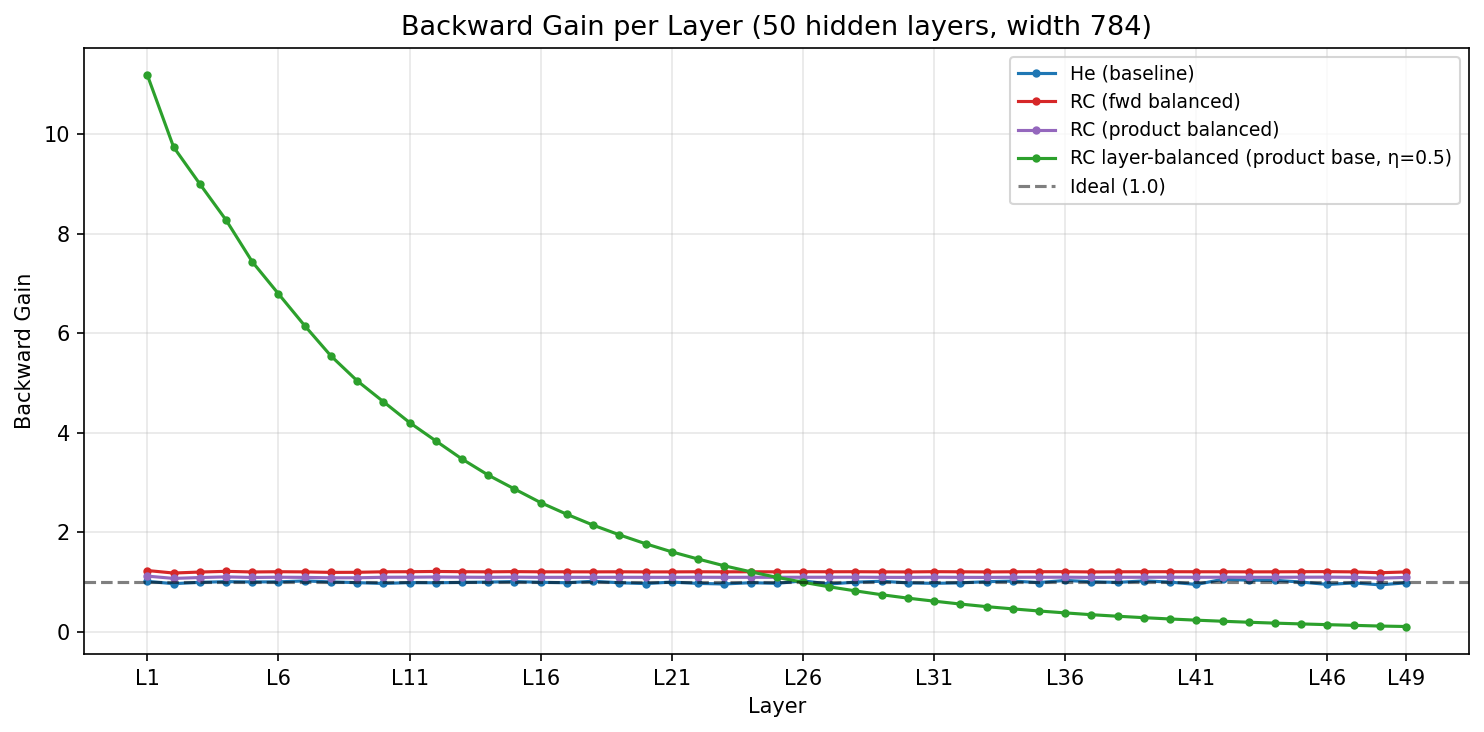
\includegraphics[width=0.92\textwidth]{backward_gain.png}
  \caption{Backward gain per layer.  Layer-balanced (green) has moderate backward gain $\approx 1.05$.}
  \label{fig:bwd-gain}
\end{figure}

\subsection{Gain product per layer}
\begin{figure}[H]
  \centering
  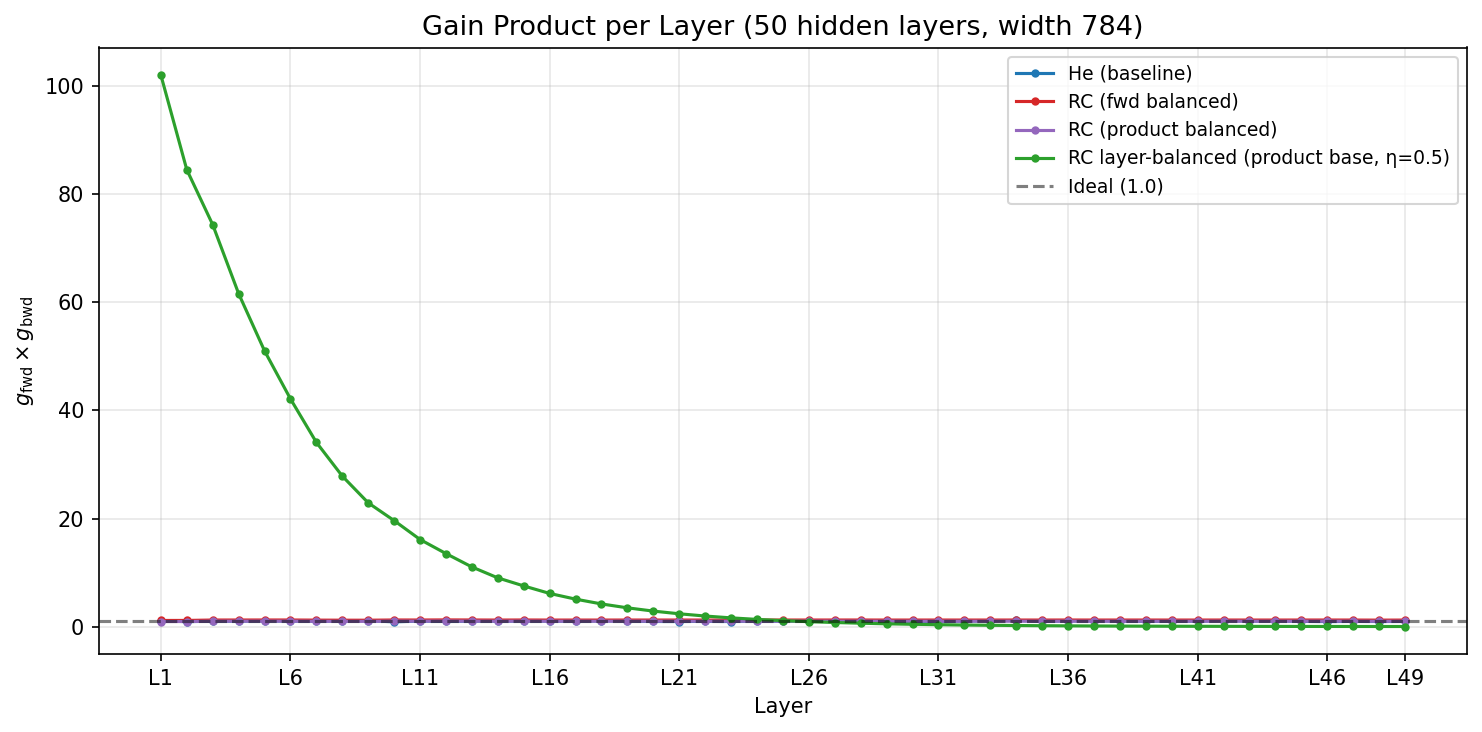
\includegraphics[width=0.92\textwidth]{gain_product.png}
  \caption{Gain product per layer.  Product-balanced and layer-balanced both sit near~1.0.}
  \label{fig:gain-product}
\end{figure}

\subsection{Gradient row norms}
\begin{figure}[H]
  \centering
  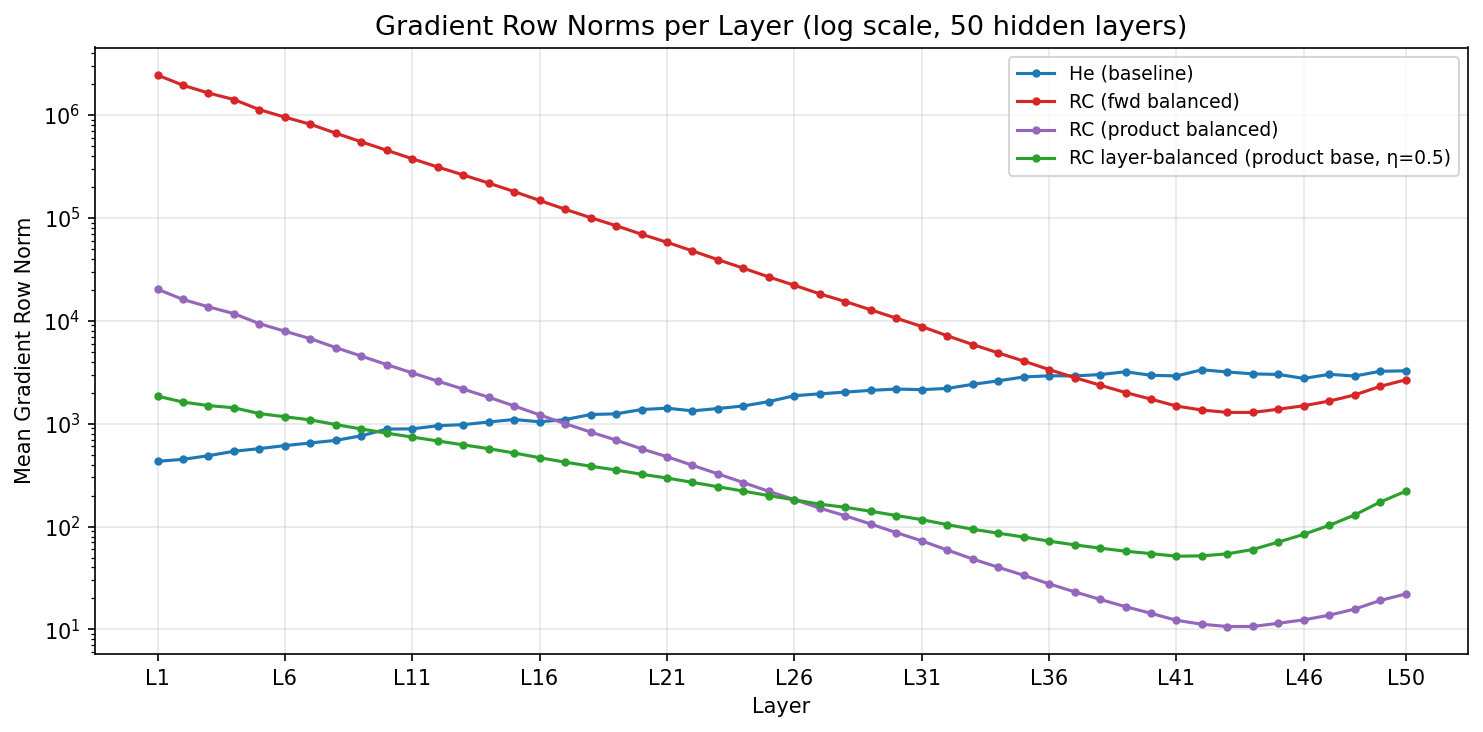
\includegraphics[width=0.92\textwidth]{gradient_norms.png}
  \caption{Gradient row norms (log scale).  He is nearly flat.  Layer-balanced (green) has moderate slope.
           Uniform RC variants (red, purple) have steep decay.}
  \label{fig:grad-norms}
\end{figure}


%======================================================================
\section{Geometry Preservation (k-NN Accuracy)}
\label{sec:geometry}

\begin{table}[H]
\centering
\caption{k-NN accuracy vs.\ depth.  Chance level $= 0.10$.}
\label{tab:knn}
\begin{tabular}{l c c c c}
\toprule
Initializer & 5\,L & 10\,L & 15\,L & 20\,L \\
\midrule
He (baseline) & 0.829 & 0.800 & 0.784 & \textbf{0.752} \\
RC fwd-balanced & 0.810 & 0.636 & 0.356 & 0.270 \\
RC product-balanced & 0.810 & 0.636 & 0.356 & 0.269 \\
RC layer-bal ($\eta\!=\!0.5$) & 0.810 & 0.636 & 0.356 & 0.270 \\
\bottomrule
\end{tabular}
\end{table}

\begin{figure}[H]
  \centering
  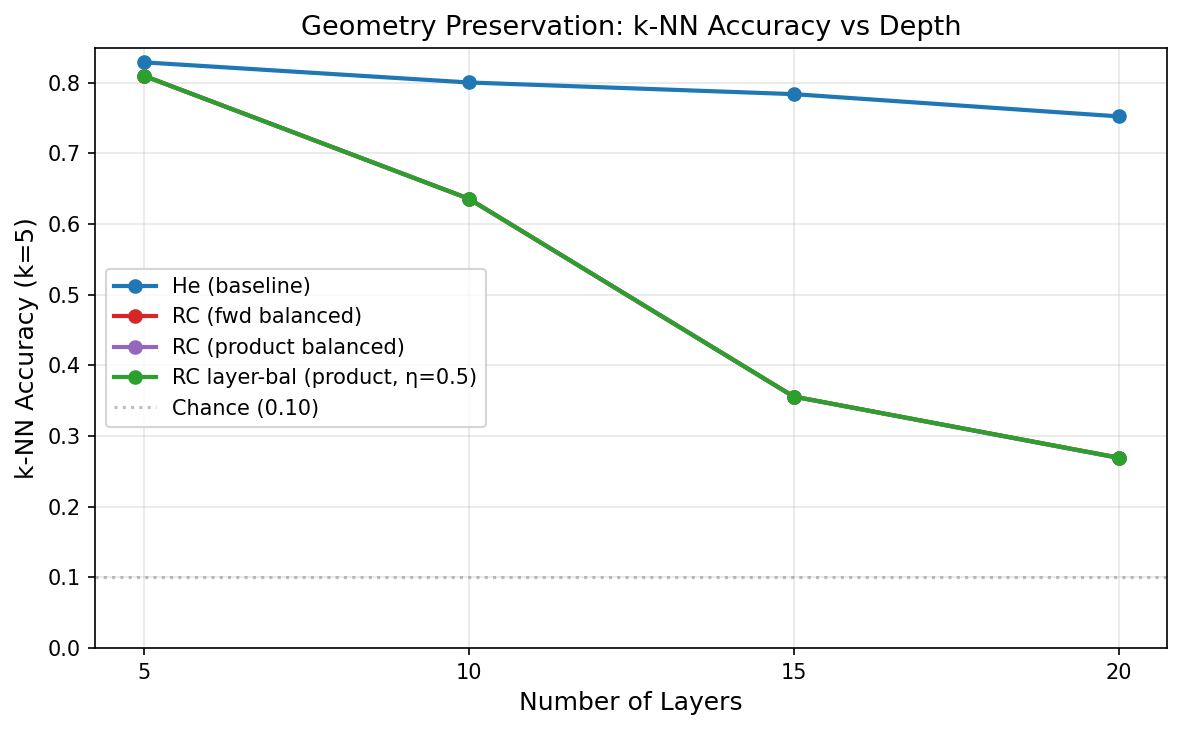
\includegraphics[width=0.7\textwidth]{knn_accuracy.png}
  \caption{k-NN accuracy vs.\ depth.  All three RC variants are identical.}
  \label{fig:knn}
\end{figure}

\begin{remark}
  All row-centered variants --- uniform or layer-balanced, regardless of
  variance --- produce identical k-NN curves.  The constraint
  $\sum_j W_{ij} = 0$ makes the neuron blind to the mean activation.
  This DC-blindness is what destroys class structure, and it is
  completely independent of the variance scale~$s$.
\end{remark}


%======================================================================
\section{The Pareto Frontier}
\label{sec:pareto}

\begin{theorem}[Pareto budget]
\label{thm:pareto}
For the $\eta$-schedule \eqref{eq:eta-schedule}:
\begin{align}
  G(\eta) &= r^{-(1-\eta)(L-1)} \quad\text{(gradient ratio)}, \\
  V(\eta) &= r^{-\eta(L-1)} \quad\text{(variance ratio)}.
\end{align}
Their product is independent of~$\eta$:
\begin{equation}\label{eq:pareto}
  \boxed{\;G(\eta) \cdot V(\eta) = r^{-(L-1)}.\;}
\end{equation}
\end{theorem}
\begin{proof}
  $G \cdot V = r^{-(1-\eta)(L-1)} \cdot r^{-\eta(L-1)}
             = r^{-[(1-\eta)+\eta](L-1)} = r^{-(L-1)}$.
\end{proof}

\begin{table}[H]
\centering
\caption{Pareto budget at various depths.}
\label{tab:budget}
\begin{tabular}{c c}
\toprule
Depth $L$ & Budget $r^{-(L-1)}$ \\
\midrule
10  & $5.6\times$ \\
20  & $38\times$ \\
50  & $11{,}943\times$ \\
100 & $1.7 \times 10^8$ \\
\bottomrule
\end{tabular}
\end{table}

Given a target gradient ratio~$T$, the required~$\eta$ is:
\begin{equation}\label{eq:eta-adaptive}
  \eta^{\ast}(L, T) = \max\!\left(0,\;\; 1 - \frac{\ln T}{(L-1) \cdot \ln(1/r)}\right).
\end{equation}


%======================================================================
\section{Beyond Row Centering: What Are the Options?}
\label{sec:beyond}

The results above establish that row centering faces two fundamental
barriers for deep networks:
\begin{enumerate}[nosep]
  \item \textbf{Gradient barrier}: the Pareto budget $r^{-(L-1)}$ grows
        exponentially with depth.
  \item \textbf{Geometry barrier}: the DC-blindness ($\sum_j W_{ij} = 0$)
        destroys class structure independently of variance.
\end{enumerate}

Both barriers stem from the same structural factor $r = \sqrt{(\pi-1)/\pi}$.
To escape them, we must either change the weight constraint or change the
nonlinearity.

\subsection{The ReLU kernel contraction: an intrinsic limit}

Even without row centering, every ReLU layer contracts angles.  The
arc-cosine kernel gives the expected cosine similarity after one layer:
\begin{equation}\label{eq:kernel}
  \hat{K}(\alpha) = \frac{1}{\pi}\bigl(\sin\alpha + (\pi - \alpha)\cos\alpha\bigr),
\end{equation}
with distortion $D(\alpha) = \hat{K}(\alpha) - \cos\alpha > 0$ for all
$\alpha \in (0, \pi)$.  This contraction is a property of ReLU itself ---
no initialization can eliminate it (Chapter~6 of the main report proves
that no pointwise nonlinearity achieves $D(\alpha) = 0$ everywhere).

\subsection{Orthogonal He: the current practical winner}

Orthogonal initialization with He scaling ($W = \sqrt{2}\,Q$, where $Q$
is from QR decomposition):
\begin{itemize}[nosep]
  \item $g_{\mathrm{fwd}} \approx 1$, $g_{\mathrm{bwd}} \approx 1$
        (no gradient trap, no coupling).
  \item Same expected kernel as He --- the systematic contraction $D(\alpha)$
        is identical.
  \item k-NN accuracy: 0.662 at 20\,L vs.\ He's 0.639 --- a $\sim\!3.6\%$
        improvement from reduced variance (better concentration around the
        expected kernel).
  \item No row centering $\Rightarrow$ no DC-blindness $\Rightarrow$ no
        geometry destruction via the 71$^\circ$ fixed-point mechanism.
\end{itemize}

The improvement of orthogonal over He is small because it only reduces
the \emph{variance} of the kernel estimate, not the \emph{expected}
distortion $D(\alpha)$.

\subsection{Batch normalization: a dynamic alternative}

The advisor's observation that batch normalization (BN) works well for
CNNs but not for fully connected networks is relevant here.  BN performs
at each layer:
\[
  \hat{a}_j = \frac{a_j - \mu_B}{\sigma_B},
\]
where $\mu_B$ and $\sigma_B$ are the batch mean and standard deviation.
This is effectively a \emph{data-dependent} centering and rescaling of
activations --- precisely what row centering tries to achieve via the
\emph{weights}.

The critical difference: BN centers the \emph{actual activations}
(adapting to the data at each layer), while row centering constrains
the \emph{weights} (a fixed structural constraint independent of data).
BN can re-center without losing signal because it also rescales;
row centering loses signal because the rescaling cannot recover the
DC information that was structurally eliminated.

This suggests that the CNN/FC comparison experiments (with and without BN)
may reveal whether BN's dynamic centering avoids the Pareto frontier
that static row centering cannot escape.

\subsection{Summary of candidates}

\begin{table}[H]
\centering
\caption{Comparison of initialization approaches for deep ReLU networks.}
\label{tab:candidates}
\begin{tabular}{l c c c}
\toprule
Approach & Gradient stability & Geometry & Limitation \\
\midrule
He                    & $g_{\mathrm{fwd}} = g_{\mathrm{bwd}} = 1$ & Degrades (0.64 at 20\,L) & ReLU contraction \\
Orthogonal He         & $g_{\mathrm{fwd}} = g_{\mathrm{bwd}} = 1$ & Slightly better (0.66)    & Same expected kernel \\
RC product-balanced   & Product $= 1$                              & Collapses (0.27 at 20\,L) & Pareto + DC-blindness \\
RC layer-balanced     & Ratio $36\times$ at $L\!=\!50$             & Collapses (0.27 at 20\,L) & Same barriers \\
BatchNorm (dynamic)   & Adaptive                                   & Unknown (to test)         & Not an initializer \\
\bottomrule
\end{tabular}
\end{table}


%======================================================================
\section{Conclusion}
\label{sec:conclusion}

\subsection{Results}
\begin{enumerate}
  \item The product-balanced variance $v^{\ast} = 2\sqrt{\pi/(\pi-1)}/d \approx 2.422/d$
        achieves $g_{\mathrm{fwd}} \cdot g_{\mathrm{bwd}} = 1$ exactly.
  \item Combined with per-layer scaling ($\eta = 0.5$), the gradient ratio
        at $L = 50$ improves from $1902\times$ to $36\times$.
  \item The Pareto budget $G(\eta) \cdot V(\eta) = r^{-(L-1)}$ is a fundamental
        limit that grows exponentially with depth.
  \item Geometry (k-NN accuracy) is identical for all RC variants ---
        the variance is irrelevant.
  \item Orthogonal He remains the practical winner for geometry + gradients,
        though it cannot eliminate the intrinsic ReLU kernel contraction.
\end{enumerate}

\subsection{Next steps}
\begin{itemize}
  \item CNN and FC experiments with and without BatchNorm, using He and
        candidate initializers, on Fashion-MNIST and CIFAR-10.
  \item Investigate whether BN's dynamic centering avoids the Pareto
        frontier that static row centering cannot escape.
\end{itemize}

\end{document}
